%31/03 - Carlos Alaíz 
\chapter{Modelos lineales, métodos de Kernel y redes neuronales}
\section{Modelos lineales de regresión}
El aprendizaje supervisado es la creación de un modelo que prediga la salida en base a unas entradas, partiendo de un histórico con parejas entrada-salida. Dentro de esto aparece la regresión, donde se quiere predecir un valor continuo. 

Los elementos de un problema de aprendizaje supervisado son:
\begin{itemize}
\item Datos: parejas entrada-salida
\item Características: atributos
\item Objetivo: la salida real, las etiquetas, la salida asociada
\item Modelo: una función matemática de x a y que proporciona la salida. Puede tener varios parámetros $\Theta$.
\item Algoritmo de aprendizaje: procedimiento para la obtención del modelo en base a los datos.
\end{itemize}

El enfoque más sencillo de la regresión es un modelo constante, ignorando la entrada. Así, se define la salida como una combinación lineal de entradas, creando un modelo lineal. La ventaja es que es simple, robusto, interpretable, fácil de entrenar y fácil de predecir. La desventaja es que sea demasiado limitado y un subajuste a los datos.

\subsection{Regresión lineal 1-dimensional}
El caso más simple tiene un solo dato de valores reales. El modelo lineal simple sería una línea recta con parámetros $\Theta = \{b, w\}$, siendo $b$ el sesgo y $w$ la pendiente de la recta. Así, el modelo se definiría como
$$f_{\Theta} = b + wx$$

Ejercicio: dado este modelo lineal con $b=1$ y $w=2$, computa la salida del modelo para $x=2$ y para $x=-1$.
$$1 + 2 \cdot 2 = 1 + 4 = 5$$
$$1 + 2 \cdot -1 = 1 - 2 = -1 $$

Se necesita un procedimiento que determine el sesgo y la pendiente para optimizar la calidad del modelo. Se pueden utilizar dos perspectivas para definir la calidad: 
\begin{itemize}
\item En base al error: medida sobre cómo de bien se ajusta el modelo a los datos de entrenamiento
\item En base a la complejidad: un término de regulación que penaliza la complejidad del modelo
\end{itemize}

Se define el residuo como la diferencia entre lo que se debería haber predicho y lo que el modelo ha predicho. El error cuadrático sería la esperanza de los residuos al cuadrado. Es decir, sobre el conjunto de datos de entrenamiento, se mide el error, se suma y se eleva al cuadrado. Esto es una medida automática de cuánto se confunde el modelo. También se puede calcular el error absoluto con el valor absoluto en lugar del error cuadrado. 

Ejercicio: calcular MAE y MSE del modelo anterior con $b=1$ y $w=2$ con los pares (2,4) y (-1,1).
$$f_{\Theta} = 1 + 2 \cdot 2 = 1 + 4 = 5 \neq 4$$
$$f_{\Theta} = 1 + 2 \cdot -1 = 1 - 2 = -1 \neq 1$$
$$r = -1, 2$$
$$MAE = 1/2 \cdot (1 + 2) = 1/2 \cdot 3 = 1.5$$
$$MSE = 1/2 \cdot (1^2 + 2^2) = 1/2 \cdot (1 + 4) = 2.5$$

%01/04 - Carlos
\subsubsection{Optimización}
Optimizar hace referencia a encontrar la mejor solución posible respecto a algún criterio. 

En un modelo lineal, hay que elegir una métrica que generalmente es el error cuadrático. Esto se debe a que es diferenciable (se puede calcular la derivada) y tiene sentido geométricamente. En el algoritmo, la optimización sería los valores de $b$ y $w$ que hacen que el error cuadrático sea mínimo.

En resumen, la línea de regresión por mínimos cuadrados se obtiene resolviendo
$$\min_{b, w \in \mathbb{R}} \left\{ \frac{1}{N} \sum_{i=1}^{N} \left( y_i - (b + w x_i) \right)^2 \right\}$$
Los elementos auxiliares son:
$$
\bar{y} = \frac{1}{N} \sum_{i=1}^{N} y_i \quad \text{(Mean Target)}, \quad
\bar{x} = \frac{1}{N} \sum_{i=1}^{N} x_i \quad \text{(Mean Feature)},
$$
$$
\hat{y}_i = y_i - \bar{y} \quad \text{(Centred Target)}, \quad
\hat{x}_i = x_i - \bar{x} \quad \text{(Centred Feature)}.
$$

Ejercicio: dado los siguientes pares de datos (0,4), (1,6), (2,4), (3,6), (4,8), computa:
\begin{itemize}
\item El valor de $\bar{x}$ y $\bar{y}$: 
$$\bar{x} = (0 + 1 + 2 + 3 + 4)/5 = 10/5 = 2$$
$$\bar{y} = (4 + 6 + 4 + 6 + 8)/5 = 28/5 = 5.6$$

\item El valor de $\hat{x}_i$ y $\hat{y}_i$:
$$\hat{x}_1 = 0 - 2 = -2 \quad \hat{y}_1 = 4 - 5.6 = -1.6$$
$$\hat{x}_2 = 1 - 2 = -1 \quad \hat{y}_2 = 6 - 5.6 = 0.4$$
$$\hat{x}_3 = 2 - 2 = 0 \quad \hat{y}_3 = 4 - 5.6 = -1.6$$
$$\hat{x}_4 = 3 - 2 = 1 \quad \hat{y}_4 = 6 - 5.6 = 0.4$$
$$\hat{x}_5 = 4 - 2 = 2 \quad \hat{y}_5 = 8 - 5.6 = 2.4$$

\item El valor de $w^*$ y $b^*$:
$$w^* = \frac{\sum^N_{i=1} \hat{x}_i\hat{y}_i}{\sum^N_{i=1} \hat{x}_i\hat{x}_i} = \frac{3.2 - 0.4 + 0 + 0.4 + 4.8 }{4 + 1 + 0 + 1 + 4} = \frac{8}{10} = 0.8$$
$$b^* = \bar{y} - w^*\bar{x} = 5.6 - 0.8 \cdot 2 = 4$$

\item El valor de MSE:
$$MSE = \frac{1}{N} \sum^N_{i=1} (y_i - (b + wx_i))^2$$
$$\frac{1}{5} \cdot ((4 - (4 + 0.8\cdot 0)^2 + 6 - (4 + 0.8\cdot 1)^2 + 4 - (4 + 0.8\cdot 2)^2 + 6 - (4 + 0.8\cdot 3)^2 + 8 - (4 + 0.8\cdot 4))^2$$
$$\frac{1}{5} \cdot (0 + 1.44 + 2.56 + 0.16 + 0.64) = \frac{1}{5} \cdot 4.8 = 0.96$$
\end{itemize}

\subsection{Regresión lineal múltiple}
Por simplicidad, $\mathcal{X} = \mathbb{R}^d$. Los datos se representan como $D = \{ (x_i, y_i) \}_{i=1}^N$, donde $x_i = (x_{i,1}, x_{i,2}, \ldots, x_{i,d}) \in \mathbb{R}^d$ y $y_i \in \mathbb{R}$.

El modelo lineal correspondiente es un hiperplano, con parámetros $\theta = \{ b, w \}$.
\begin{itemize}
\item $b \in \mathbb{R}$ es el término de intercepción o sesgo.
\item $w = (w_1, w_2, \ldots, w_d) \in \mathbb{R}^d$ es el vector normal del hiperplano.
\item El modelo se define como:    
    $$f_\theta (\mathbf{x}) = b + w^\top \mathbf{x} = b + \sum_{i=1}^d w_i x_i.$$
\end{itemize}

El algoritmo de aprendizaje determinará $b$ y $w$ utilizando $D$.

Ejercicio: dado un modelo lineal bidimensional con parámetros $\Theta = \{ b, \vec{w}\}$ con $b = 1$ y $\vec{w} = (1,2)^T$. Computa la salida del modelo para $\vec{x} = (1,1)^T$:
$$1 + (1 \cdot 1 + 1 \cdot 2) = 4$$
 Computa la salida del modelo para $\vec{x} = (-1,0)^T$:
 $$1 + (1 \cdot -1 + 0 \cdot 2) = 0$$

\subsubsection{Ecuaciones lineales}
Se necesita un procedimiento para determinar el sesgo $b $ y el vector $\mathbf{w}$.

Un primer enfoque es intentar igualar todos los pares entrada-salida $(x_i, y_i)$, $i = 1, \ldots, N$. Específicamente:
$$
\begin{cases}
b + \mathbf{w}^T x_1 = y_1 \\
b + \mathbf{w}^T x_2 = y_2 \\
\vdots \\
b + \mathbf{w}^T x_N = y_N
\end{cases}
\equiv 
\begin{cases}
b + w_1 x_{1,1} + w_2 x_{1,2} + \cdots + w_d x_{1,d} = y_1 \\
b + w_1 x_{2,1} + w_2 x_{2,2} + \cdots + w_d x_{2,d} = y_2 \\
\vdots \\
b + w_1 x_{N,1} + w_2 x_{N,2} + \cdots + w_d x_{N,d} = y_N
\end{cases}
$$

La siguiente notación matricial puede simplificar las ecuaciones:
$$
\mathbf{X} =
\begin{pmatrix}
x_{1,1} & x_{1,2} & \cdots & x_{1,d} \\
x_{2,1} & x_{2,2} & \cdots & x_{2,d} \\
\vdots & \vdots & \ddots & \vdots \\
x_{N,1} & x_{N,2} & \cdots & x_{N,d}
\end{pmatrix}
;\quad \tilde{\mathbf{X}} =
\begin{pmatrix}
1 & x_{1,1} & \cdots & x_{1,d} \\
1 & x_{2,1} & \cdots & x_{2,d} \\
\vdots & \vdots & \ddots & \vdots \\
1 & x_{N,1} & \cdots & x_{N,d}
\end{pmatrix}
;\quad \mathbf{y} =
\begin{pmatrix}
y_1 \\
y_2 \\
\vdots \\
y_N
\end{pmatrix}
;\quad \tilde{\mathbf{w}} =
\begin{pmatrix}
b \\
w_1 \\
\vdots \\
w_d
\end{pmatrix},
$$

donde $\mathbf{X} \in \mathbb{R}^{N \times d}$ es la matriz de datos, $ \tilde{\mathbf{X}} \in \mathbb{R}^{N \times (d+1)}$ es la matriz de datos con un término constante, $\mathbf{y} \in \mathbb{R}^N$ es el vector de objetivos y $\tilde{\mathbf{w}} \in \mathbb{R}^{d+1}$ es el vector de pesos que incluye el intercepto.

El sistema de ecuaciones se convierte en $\tilde{\vec{X}}\tilde{\vec{w}} = \vec{y}$. Como $\tilde{\vec{X}} \in \real^{N \times (d + 1)}, \tilde{\vec{w}} \in \real^{d + 1}$ y $\vec{y} \in \real^N$, tenemos $N$ ecuaciones y $d + 1$ incógnitas. Normalmente, $N >> d+1$ y el sistema está \textbf{sobredeterminado}.

\subsubsection{Calidad del modelo}
Se define con el término de error y de complejidad, al igual que en el caso de una sola dimensión. Los residuos son la desviación de la salida con respecto a la predicción. El error cuadrático y el error absoluto se definen igual que antes.

Para el $i$-ésimo patrón, el \textbf{residual} se define como:
$$
r_i = y_i - f_\theta(\mathbf{x}_i) = y_i - (b + \mathbf{w}^\intercal\mathbf{x}_i).
$$

El \textbf{Error Cuadrático Medio} se calcula como:
$$
\text{MSE}(b, \mathbf{w}) = \mathbb{E}\left[R^2\right] \approx \frac{1}{N} \sum_{i=1}^{N} \big(y_i - (b + \mathbf{w}^\intercal\mathbf{x}_i)\big)^2.
$$

$$
\text{MAE}(b, \mathbf{w}) = \mathbb{E}\left[|R|\right] \approx \frac{1}{N} \sum_{i=1}^{N} \left|y_i - (b + \mathbf{w}^\intercal\mathbf{x}_i)\right|.
$$

Ejercicio: dado un modelo lineal bidimensional con parámetros $\Theta = \{b, \vec{w}\}$, con $b=1$ y $\vec{w} = (1,2)^T$, y los datos siguientes datos para $x_{i,1}$, $x_{i,2}$ y $y_i$, computa MAE y MSE.
Para un modelo lineal bidimensional:
$$f(x_1, x_2) = b + w_1x_1 + w_2x_2$$
En el enunciado nos dicen b y w, por lo que la fórmula queda en:
$$f(x_1, x_2) = 1 + 1 x_1 + 2 x_2$$
Ahora tenemos dos datos, por lo que calculamos las salidas predichas:
$$f_1 = 1 + 1 + 2 = 4$$
$$f_2 = 1 - 1 + 0 = 0 \neq 2$$
Los residuos son 0 y 2. Por tanto, los residuos cuadrados son 0 y 4. Calculando la media, $MAE = 1$ y $MSE = 2$. 

\subsubsection{Optimización basada en gradiente: problemas multidimensionales}
En muchas dimensiones, la derivada se generaliza con el gradiente, que es un vector de derivadas parciales. El gradiente define el hiperplano tangente. 

\subsubsection{Entrenamiento de un modelo lineal}
Usualmente se utiliza como función de error el MSE al ser diferenciable y corresponderse a la distancia entre los vectores de predicción y de salida esperada. Se busca minimizar este error, calculando para cada entrada la salida correspondiente y viendo el error.

El problema de optimización para encontrar los parámetros óptimos se formula como:

$$
\min_{\substack{b \in \mathbb{R} \\ \mathbf{w} \in \mathbb{R}^d}} \left\{ \text{MSE}(b, \mathbf{w}) \right\} = \min_{\substack{b \in \mathbb{R} \\ \mathbf{w} \in \mathbb{R}^d}} \left\{ \frac{1}{N} \sum_{i=1}^{N} \big(y_i - (b + \mathbf{w}^\intercal\mathbf{x}_i)\big)^2 \right\} \equiv \min_{\tilde{\mathbf{w}} \in \mathbb{R}^{d+1}} \left\{ (\mathbf{y} - \tilde{\mathbf{X}}\tilde{\mathbf{w}})^\top (\mathbf{y} - \tilde{\mathbf{X}}\tilde{\mathbf{w}}) \right\}.
$$

Para encontrar el punto óptimo $\tilde{\mathbf{w}}^*$, calculamos el gradiente e igualamos a cero:

$$\nabla_{\tilde{\mathbf{w}}} \text{MSE}(\tilde{\mathbf{w}})\big|_{\tilde{\mathbf{w}}=\tilde{\mathbf{w}}^*} = \mathbf{0} \implies 2\tilde{\mathbf{X}}^\top(\mathbf{y} - \tilde{\mathbf{X}}\tilde{\mathbf{w}}^*) = \mathbf{0}
$$

Esto conduce al sistema de ecuaciones normales:

$$\tilde{\mathbf{X}}^\top \mathbf{y} - \tilde{\mathbf{X}}^\top \tilde{\mathbf{X}}\tilde{\mathbf{w}}^* = \mathbf{0} \\
\implies \tilde{\mathbf{X}}^\top \tilde{\mathbf{X}}\tilde{\mathbf{w}}^* = \tilde{\mathbf{X}}^\top \mathbf{y}
$$

Finalmente, la solución óptima (si $\tilde{\mathbf{X}}^\top \tilde{\mathbf{X}}$ es invertible) es:

$$
\tilde{\mathbf{w}}^* = (\tilde{\mathbf{X}}^\top \tilde{\mathbf{X}})^{-1} \tilde{\mathbf{X}}^\top \mathbf{y} \quad \text{(Mínimos Cuadrados)}
$$

Caso especial: cuando $\tilde{\mathbf{X}}^\top \tilde{\mathbf{X}}$ es invertible y $N = d+1$, se simplifica a:
$$
\tilde{\mathbf{w}}^* = \tilde{\mathbf{X}}^\top \mathbf{y}
$$

En resumen, el modelo de mínimos cuadrados lineales es la solución del siguiente problema de optimización:
$$
\min_{\begin{subarray}{c} 
    b \in \mathbb{R} \\
    \mathbf{w} \in \mathbb{R}^d 
\end{subarray}} \left\{ 
    \frac{1}{N} \sum_{i=1}^{N} \big(y_i - (b + \mathbf{w}^{\intercal} \mathbf{x}_i)\big)^2 
\right\}.
$$

La solución óptima viene dada por:
$$
\begin{pmatrix} b^* \\ \mathbf{w}^* \end{pmatrix} = 
\tilde{\mathbf{w}}^* = 
\tilde{\mathbf{X}}^{\dagger} \mathbf{y} = 
\begin{bmatrix} \mathbf{1} & \mathbf{X} \end{bmatrix}^{\dagger} \mathbf{y},
$$

donde:
\begin{itemize}
\item $\tilde{\mathbf{X}} = \begin{bmatrix} \mathbf{1} & \mathbf{X} \end{bmatrix}$ es la matriz de diseño aumentada
\item $\dagger$ denota la pseudoinversa de Moore-Penrose
\item $\mathbf{1}$ es un vector columna de unos
\end{itemize}

\subsection{Resumen: modelos lineales para regresión}
Un problema de regresión es un problema supervisado con objetivos continuos. Un modelo de regresión sencillo pero útil es el modelo lineal. La predicción es una combinación lineal de las características. Para entrenar el modelo lineal, se suele resolver un problema de optimización. El MSE suele utilizarse para medir la calidad del modelo. Es una elección natural. El problema resultante puede resolverse de forma cerrada utilizando el pseudoinverso de la matriz de datos.

%07/04 - Carlos
\section{Modelos lineales de clasificación}
Un problema de clasificación es un problema de aprendizaje supervisado en el que las salidas son discretas. Ejemplos son predecir si un paciente padece o no una determinada enfermedad en función de datos médicos, distinguir la especie de un pez capturado utilizando los datos proporcionados por varios sensores o discernir el tipo de objeto que aparece en una imagen.

Los elementos de un problema de aprendizaje supervisado son:
\begin{itemize}
\item Datos: conjunto de pares entrada-salida
\item Características: vector de atributos (variables independientes/de entrada, covariables...)
\item Etiquetas: objetivo (variable dependiente, resultado...)
\item Modelo: asignación del espacio de entrada al de salida
\item Algoritmo de aprendizaje: procedimiento para obtener un modelo basado en los datos
\end{itemize}

\subsection{Clasificación binaria lineal}
El escenario de clasificación más importante es cuando M = 2 (clasificación binaria).
Si M > 2, existen técnicas de codificación para transformar el problema en varios subproblemas binarios.
Las clases suelen denominarse C0 y C1, y se representan con una codificación 0/1 (o -1/1). Las etiquetas se transforman en:
$$t_i = \begin{cases}
0 \quad \text{if } y_i = \mathcal{C}_0 \\
1 \quad  \text{if } y_i = \mathcal{C}_1
\end{cases}
$$

Los enfoques más simples de clasificación son:
\begin{itemize}
\item Ignorar la entrada: modelo constante (normalmente, clase mayoritaria).
\item Definir la salida como una combinación lineal de las entradas más una transformación: modelo lineal. Es simple, robusto (varianza pequeña), interpretable, fácil de entrenar y fácil de predecir. No obstante, tiene flexibilidad limitada y un ajuste insuficiente (gran sesgo).
\end{itemize}

Por simplicidad, $\mathcal{X}=\mathbb{R}^{d}$.
Los datos se convierten en $\mathcal{D}=\{(x_{i},t_{i})\}_{i=1}^{N}$, donde $x_{i}=(x_{i,1},x_{i,2},\ldots,x_{i,d})\in\mathbb{R}^{d}$ y $t_{i}\in\{0,1\}$.
El modelo lineal correspondiente es un hiperplano, con parámetros $\boldsymbol{\theta}=\{b,\mathbf{w}\}$.

\begin{itemize}
    \item $b\in\mathbb{R}$ es el término de intercepción o sesgo.
    
    \item $\mathbf{w}=(w_{1},w_{2},\ldots,w_{d})\in\mathbb{R}^{d}$ es el vector normal del hiperplano.
    
    \item El modelo se define como:
    \[f_{\boldsymbol{\theta}}(\mathbf{x})=\begin{cases}
    0 & \text{si } b+\mathbf{w}^{\intercal}\mathbf{x}<0, \\
    1 & \text{si } b+\mathbf{w}^{\intercal}\mathbf{x}\geq 0.
    \end{cases}\]
    
    \item El hiperplano divide el espacio en dos mitades, una para la clase $\mathcal{C}_{0}$ y la otra para la clase $\mathcal{C}_{1}$.
\end{itemize}

El \textbf{algoritmo de aprendizaje} determinará $b$ y $\mathbf{w}$ utilizando $\mathcal{D}$.

Ejercicio: dado un modelo de clasificación lineal binario bidimensional con parámetros $\theta = \{b, \vec{w}\}$, con $b = 1$ y $\vec{w} = (1, 2)^T$:
\begin{itemize}
\item Calcula la salida del modelo para $\vec{x}_1 = (1,1)$:

$$1 + 1 \cdot 1 + 2 \cdot 1 = 4 \rightarrow f_{\theta}(\vec{x}) = \mathcal{C}_1$$

\item Calcula la salida del modelo para $\vec{x}_2 = (1,-2)$:

$$1 + 1 \cdot 1 + 2 \cdot (-2) = -2 \rightarrow f_{\theta}(\vec{x}) = \mathcal{C}_0$$

\item Calcula la salida del modelo para $\vec{x}_3 = (0,0)$:

$$1 + 1 \cdot 0 + 2 \cdot 0 = 1 \rightarrow f_{\theta}(\vec{x}) = \mathcal{C}_1$$
\end{itemize}

\subsubsection{Calidad del modelo}
Se necesita un procedimiento para determinar el sesgo $b$ y el vector $w$, optimizando la calidad del modelo. Hay que definir la calidad del modelo. Normalmente desde dos puntos de vista:
\begin{itemize}
\item Ajuste: Un término de aptitud $\mathcal{F_D}(\theta)$ mide lo bien que el modelo se ajusta a los datos de entrenamiento.
\item Complejidad: Un término de regularización $\mathcal{R}(\theta)$ penaliza la complejidad del modelo
\end{itemize}

\textbf{Predicción Correcta} Para el $i$-ésimo patrón,

\[c_i = 
\begin{cases} 
0 & \text{si } t_i \neq f_0(\mathbf{x}_i) \\ 
1 & \text{si } t_i = f_0(\mathbf{x}_i) 
\end{cases}
= 
\begin{cases} 
0 & \text{si } (t_i = 0, b + \mathbf{w}^\intercal \mathbf{x}_i \geq 0) \text{ o } (t_i = 1, b + \mathbf{w}^\intercal \mathbf{x}_i < 0), \\ 
1 & \text{si } (t_i = 0, b + \mathbf{w}^\intercal \mathbf{x}_i < 0) \text{ o } (t_i = 1, b + \mathbf{w}^\intercal \mathbf{x}_i \geq 0). 
\end{cases}\]

\textbf{Precisión} Acc$(b, \mathbf{w}) = \mathbb{E}[C] \approx \frac{1}{N} \sum_{i=1}^{N} c_i$.

Ejercicio: dado un modelo de clasificación binario lineal bidimensional con los parámetros $\theta = (b, \vec{w})$ con $b=1$ y $\vec{w} = (1,2)^T$ y los siguientes datos, computa la precisión:
$$(1,1; 1) \rightarrow 1 + 1 \cdot 1 + 1 \cdot 2 = 4 \rightarrow 1 = 1$$
$$(1,-2; 0) \rightarrow 1 + 1 \cdot 1 + 2 \cdot -2 = -2 \rightarrow 0 = 0$$
$$(0,0; 0) \rightarrow 1 + 1 \cdot 0 + 2 \cdot 0 = 1 \rightarrow 1 \neq 0$$
$$Accuracy = 2/3 \approx 66.67$$

%08/04 - Carlos
La opción más habitual para evaluar el modelo es la \textbf{precisión}. Es una medida sensata e intuitiva. No es convexa, no es diferenciable y es discontinua.
Optimizar la precisión es un problema que (en general) no puede abordarse directamente. 

Una idea alternativa podría ser entrenar un \textbf{modelo de regresión lineal} con etiquetas -1/1. La etiqueta predicha se determina tomando el signo de la salida. El problema de esto es que con datos asimétricos, el modelo minimiza el error cuadrático, pudiendo mover la frontera. Se penaliza tener valores demasiado positivos o demasiado negativos, intentando ajustarse siempre a los valores 1 y -1. 

Por tanto, se necesita una medida de calidad diferente que debería ser más fácil de optimizar que la precisión. No debería penalizar los puntos alejados del límite de decisión (pero en el lado correcto). Un enfoque probabilístico puede ser útil. En particular, el marco principal es la regresión logística. El modelo lineal se utiliza para estimar la probabilidad posterior de una clase. Se utiliza una transformación sigmoidea.

Denotando por $\tilde{x} = [1, x]$ y por $\tilde{w} = [b, w]$, las probabilidades posteriores se definen como:
$$
p(C_1 \mid \tilde{x}; \tilde{w}) = \sigma(\tilde{w}^T \tilde{x}) = \frac{1}{1 + e^{-\tilde{w}^T \tilde{x}}},
$$
$$
p(C_0 \mid \tilde{x}; \tilde{w}) = 1 - p(C_1 \mid \tilde{x}; \tilde{w}) = 1 - \frac{1}{1 + e^{-\tilde{w}^T \tilde{x}}} = \frac{e^{-\tilde{w}^T \tilde{x}}}{1 + e^{-\tilde{w}^T \tilde{x}}} = \frac{1}{1 + e^{\tilde{w}^T \tilde{x}}} = \sigma(-\tilde{w}^T \tilde{x}).
$$

\begin{itemize}
    \item Si $\tilde{w}^T \tilde{x} < 0 \Rightarrow p(C_1 \mid \tilde{x}; \tilde{w}) < 0.5$: Se predice la clase $C_0$.
    \item Si $\tilde{w}^T \tilde{x} \geq 0 \Rightarrow p(C_1 \mid \tilde{x}; \tilde{w}) \geq 0.5$: Se predice la clase $C_1$.
\end{itemize}  

\begin{figure}[h]
\centering
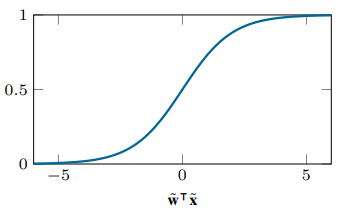
\includegraphics[width = 0.5\textwidth]{figs/sigmoidal.png}
\end{figure}  

Ejercicio: dado un modelo de clasificación binario lineal bidimensional con los parámetros $\theta = (b, \vec{w})$ con $b=1$ y $\vec{w} = (1,2)^T$ y los siguientes datos, computa la precisión:
\begin{itemize}
\item Probabilidad de $\vec{x}_1$ pertenecer a la clase $\mathcal{C}_1$ para $\vec{x}_1 = (1,1)^T$.

$$1 + 1 \cdot 1 + 2 \cdot 1 = 4$$
$$1 / (1 + e^{-4}) = 0.98$$

\item Probabilidad de $\vec{x}_2$ pertenecer a la clase $\mathcal{C}_1$ para $\vec{x}_2 = (1,-2)^T$.

$$1 + 1 \cdot 1 + 2 \cdot -2 = -2$$
$$1 / (1 + e^{2}) = 0.119$$

\item Probabilidad de $\vec{x}_3$ pertenecer a la clase $\mathcal{C}_0$ para $\vec{x}_3 = (0,0)^T$.

$$1 + 1 \cdot 0 + 2 \cdot 0 = 1$$
$$1 - (1 / (1 + e^{-1}) )= 0.2689$$
\end{itemize}

\subsubsection{Optimización: Máxima verosimilitud y entropía cruzada}

La verosimilitud de los datos es una elección común para cuantificar la calidad de un modelo probabilístico:
$$
\mathcal{L}(\mathcal{D};\tilde{\mathbf{w}}) = \prod_{i=1}^{N} p(t_i|\tilde{\mathbf{x}}_i; \tilde{\mathbf{w}}) = \prod_{i=1}^{N} \underbrace{p(C_0|\tilde{\mathbf{x}}_i; \tilde{\mathbf{w}})^{1-t_i} p(C_1|\tilde{\mathbf{x}}_i; \tilde{\mathbf{w}})^{t_i}}_{\begin{cases} 
    p(C_0|\tilde{\mathbf{x}}_i; \tilde{\mathbf{w}}) & \text{si } t_i = 0, \\ 
    p(C_1|\tilde{\mathbf{x}}_i; \tilde{\mathbf{w}}) & \text{si } t_i = 1. 
\end{cases}}
$$

El error de Entropía Cruzada (CE) se define como el logaritmo negativo de la verosimilitud:
$$
CE(\tilde{\mathbf{w}}) = -\log\mathcal{L}(\mathcal{D};\tilde{\mathbf{w}})
$$
$$
= \sum_{i=1}^{N} \left( -(1 - t_i) \log(p(C_0|\tilde{\mathbf{x}}_i; \tilde{\mathbf{w}})) - t_i \log(p(C_1|\tilde{\mathbf{x}}_i; \tilde{\mathbf{w}})) \right)
$$
$$
= \sum_{i=1}^{N} \left( -(1 - t_i) \log(1 - \sigma(\tilde{\mathbf{w}}^{T}\tilde{\mathbf{x}}_i)) - t_i \log(\sigma(\tilde{\mathbf{w}}^{T}\tilde{\mathbf{x}}_i)) \right).
$$

Ejercicio: dado un modelo de clasificación binario lineal bidimensional con los parámetros $\theta = (b, \vec{w})$ con $b=1$ y $\vec{w} = (1,2)^T$ y los siguientes datos, computa la precisión:
$$(1,1; 1) \rightarrow 1 + 1 \cdot 1 + 1 \cdot 2 = 4 $$
$$p1 = 1 / (1 + e^{-4}) = 0.98$$
$$p0 = 1 - 0.98 = 0.02$$
$$\mathcal{L} = (0.98)^1 \cdot (0.02)^0 = 0.98$$

$$(1,-2; 0) \rightarrow 1 + 1 \cdot 1 + 2 \cdot -2 = -2 $$
$$p1 = 1 / (1 + e^{2}) = 0.119$$
$$p0 = 1 - 0.119 = 0.881$$
$$\mathcal{L} = (0.881)^1 \cdot (0.119)^0 = 0.881$$

$$(0,0; 0) \rightarrow 1 + 1 \cdot 0 + 2 \cdot 0 = 1 $$
$$p1 = 1 / (1 + e^{-1}) = 0.7311$$
$$p0 = 1 - 0.2689 = 0.2689$$
$$\mathcal{L} = (0.2689)^1 \cdot (0.7311)^0 = 0.2689$$

$$ML = 0.98 \cdot 0.881 \cdot 0.2689 = 0.23$$

El CE minimizado es el máximo de ML. El algoritmo de aprendizaje para entrenar un modelo de Regresión Logística Lineal consiste en resolver el problema:
$$\min_{\tilde{\mathbf{w}} \in \mathbb{R}^{d+1}} \left\{ \mathrm{CE}(\tilde{\mathbf{w}}) \right\} = \min_{\tilde{\mathbf{w}} \in \mathbb{R}^{d+1}} \left\{ \sum_{i=1}^N \left( -(1-t_i) \log (1-\sigma(\tilde{\mathbf{w}}^{\intercal} \tilde{\mathbf{x}}_i)) - t_i \log (\sigma(\tilde{\mathbf{w}}^{\intercal} \tilde{\mathbf{x}}_i)) \right) \right\}.$$

Es convexa: no existen mínimos locales. Es diferenciable: los óptimos se caracterizan por los ceros del gradiente.

$$\nabla_{\tilde{\mathbf{w}}} \text{CE}(\tilde{\mathbf{w}})=\sum^N_{i=1} (\sigma (\tilde{\mathbf{w}}^T \tilde{\mathbf{x}}_i) - t_i) \tilde{\mathbf{x}}_i = \mathbf{0}
$$

El problema es que no siempre se puede igualar el gradiente a 0.

El Descenso Gradiente es un algoritmo de optimización simple (pero útil) que se utiliza a menudo en Aprendizaje Automático para encontrar el mínimo local.

\begin{figure}[h]
\centering
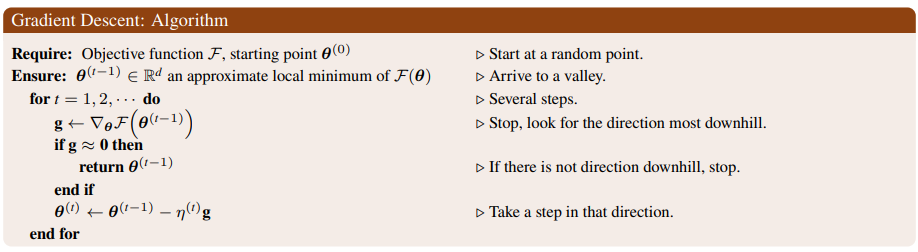
\includegraphics[width = \textwidth]{figs/gradient-descend-alg.png}
\end{figure}

El tamaño del paso $\eta^{(t)}$ debe fijarse en cada iteración t. Se trata de una cuestión crucial: Si el tamaño del paso es demasiado pequeño, el algoritmo necesitará demasiadas épocas (iteraciones) para converger y puede quedar atrapado en mínimos locales más fácilmente. Si el tamaño del paso es grande, la convergencia también será lenta. Si el tamaño del paso es demasiado grande, el descenso de gradiente sobrepasará los mínimos y divergirá. En algunos casos, se pueden calcular tamaños de paso óptimos.
Existen heurísticos que garantizan la convergencia, pero sólo a mínimos locales, y normalmente de forma lenta y zigzagueante.

%22/04 - Carlos
\section{Modelos lineales regulados}
\subsection{Introducción}
Ejercicio: dado un modelo tridimensional con los siguientes datos, define un modelo lineal $\{b, w_1, w_2, w_3\}$ con el menor MSE posible. ¿Se puede obtener una predicción perfecta?
$$(1,0,1; 2) \rightarrow 1 + 0 + 1 = 2$$
$$(1,1,1;3) \rightarrow 1 + 1 + 1 = 3$$
Es posible obtener una predicción perfecta, y hay varias posibilidades. Primero, se pueden evaluar todos los parámetros por igual con el mismo peso, o un parámetro se puede compensar con los demás. 

La complejidad del modelo se debe controlar, ya que no todas las entradas o características van a ser relevantes. Por tanto, un modelo basado en un subconjunto de características parece ser una opción sensible.

\subsubsection{Sesgo y varianza}
Suponemos un problema de regresión. Las entradas y salidas se relacionan con la ecuación $y = f^*(\vec{x}) + \epsilon$, siendo $f^*$ la función perfecta a la que no tenemos acceso. El modelo debe intentar de aproximar la función verdadera: $f \approx f^*$. La distancia entre ambas funciones se formaliza como \textbf{sesgo}. Un sesgo pequeño se puede conseguir con modelos muy flexibles y con muchos parámetros. No obstante, el modelo depende de una muestra particular de entrenamiento, $f_{\mathcal{D}}$. El modelo debe ser estable para distintos datasets $\mathcal{D}$ y $\mathcal{D}'$, de forma que $f_{\mathcal{D}} \approx f_{\mathcal{D}`}$. La estabilidad se define como \textbf{varianza}. Una varianza pequeña se consigue con modelos simples con pocos parámetros. Así, se encuentra un \textbf{trade-off}:
\begin{itemize}
\item \textbf{Error debido al sesgo:} diferencia entre la predicción esperada del modelo y el valor correcto a predecir.
\item \textbf{Error debido a la varianza:} variabilidad de la predicción del modelo para un punto de datos dado.
\end{itemize}

La regularización suele denotar el conjunto de técnicas que intentan mejorar las estimaciones desviándolas de sus valores basados en la muestra hacia valores que se consideran más "físicamente plausibles". La varianza del modelo se reduce a expensas de un sesgo potencialmente mayor.

\subsubsection{Sobreajuste y subajuste}
En el sobreajuste, el modelo resultante es excesivamente complejo para describir los datos estudiados. Se puede dar con un número limitado de datos de entrenamiento o una máquina de aprendizaje demasiado compleja (muchos parámetros libres). La varianza será grande y el sesgo pequeño.

En el subajuste, el modelo resultante es demasiado simple para describir los datos estudiados. Puede darse cuando la máquina de aprendizaje es demasiado rígida. El sesgo es grande y varianza pequeña.

La regularización viene buen cuando hay más entradas que patrones, ya que hay que asumir algo del modelo. Esto se debe a varios estimadores óptimos. Desde el punto de vista computacional, evita las inestabilidades numéricas y se evita el sobreajuste. Finalmente, el modelo sencillo mejora la parsimonia e interpretabilidad. 

\subsubsection{Aprendizaje regulado}
El aprendizaje regularizado consiste en modelos entrenados optimizando funciones objetivo de la forma:
$$\mathcal{S} = \mathcal{E_D} + \gamma \mathcal{R}$$

El término principal de la función objetivo es un término de error $\mathcal{E_D}$. Representa lo bien que el modelo se ajusta a los datos de entrenamiento $\mathcal{D}$, por ejemplo el error cuadrático medio (MSE) en regresión y la log verosimilitud negativa en clasificación. El término adicional es un término de regularización $\mathcal{R}$. Penaliza la complejidad del modelo con varios propósitos: evitar el sobreajuste, introducir conocimiento previo, y cumplir ciertas propiedades deseables. $\gamma$ es un parámetro de regularización, siendo responsable del equilibrio entre precisión y complejidad. Un $\gamma$ bajo favorece el sobreajuste. 

\subsection{Funciones reguladas}
Existen diferentes funciones de regularización $\mathcal{R}(\theta)$ que asignan a cada conjunto de parámetros $\theta$ una medida de su complejidad. Dependiendo de la función elegida, cambiará el efecto sobre $\theta$. La influencia de las funciones de regularización es especialmente clara en los modelos lineales:
\begin{itemize}
\item Cada coeficiente de w corresponde a una característica de entrada.
\item Si wi = 0, se ignora la característica i-ésima.
\item Si wi = wj, la característica i-ésima es similar a la característica j-ésima.
\end{itemize}

\subsubsection{$\ell_2$ norm}
Término clásico, conocido como regularización de Tikhonov, corresponde a la suma de los cuadrados de las entradas:
$$\mathcal{R}(\vec{w}) = ||\vec{w}||^2_2 = \sum^d_{i=1} w_i^2$$

Controla la complejidad del modelo, siendo diferenciable y fácil de optimizar. Desplaza las entradas hacia 0.

Ejercicio: Dados los siguientes modelos lineales tridimensionales, computa su $\ell_2$ norma cuadrada para comprobar cuál es más simple en base a este criterio.
$$\{w_1 = 1, w_2 = 1, w_3 = 1\} \rightarrow 1^2 + 1^2 + 1^2 = 3$$
$$\{w_1 = 3, w_2 = 0, w_3 = 0\} \rightarrow 3^2 + 0^2 + 0^2 = 9$$
$$\{w_1 = 2, w_2 = 2, w_3 = 0\} \rightarrow 2^2 + 2^2 + 0 = 8 $$
Así, el primer modelo es el más simple y el segundo el más complejo.

\subsubsection{$\ell_1$ norm}
Corresponde a la suma de los valores absolutos de las entradas:
$$\mathcal{R}(\vec{w}) = ||\vec{w}||_1 = \sum^d_{i=1} |w_i|$$

Controla la complejidad del modelo. El valor absoluto es no-diferenciable alrededor de 0, por lo que este término es más complicado de optimizar.  Empuja las entradas hacia cero obligando a que algunas de ellas sean idénticamente cero. Refuerza la dispersión (sparsity).

Ejercicio: Dados los siguientes modelos lineales tridimensionales, computa su $\ell_1$ norma para comprobar cuál es más simple en base a este criterio.
$$\{w_1 = 1, w_2 = 1, w_3 = 1\} \rightarrow 1 + 1 + 1 = 3$$
$$\{w_1 = 3, w_2 = 0, w_3 = 0\} \rightarrow 3 + 0 + 0 = 3$$
$$\{w_1 = 2, w_2 = 2, w_3 = 0\} \rightarrow 2 + 2 + 0 = 4 $$
Así, el tercer modelo es el más complejo.

%05/05 - Carlos Alaíz
\subsection{Modelos lineales regulados}
El problema de optimización para entrenar un modelo regularizado puede formularse como:
$$
\min_{\boldsymbol{\theta}} \left\{\mathcal{E}_{\mathcal{D}}(\boldsymbol{\theta}) + \gamma\mathcal{R}(\boldsymbol{\theta})\right\}.
$$

Existe una equivalencia entre este modelo sin restricciones y la siguiente formulación con restricciones:
$$
\min_{\boldsymbol{\theta}} \left\{\mathcal{E}_{\mathcal{D}}(\boldsymbol{\theta})\right\} \text{ s.t. } \mathcal{R}(\boldsymbol{\theta}) \leq c.
$$

En el caso de un modelo de regresión lineal:
$$
\min_{\mathbf{w}\in\mathbb{R}^{d}} \left\{||\mathbf{y}-\mathbf{X}\mathbf{w}||_{2}^{2} + \gamma\mathcal{R}(\mathbf{w})\right\} \equiv \min_{\mathbf{w}\in\mathbb{R}^{d}} \left\{||\mathbf{y}-\mathbf{X}\mathbf{w}||_{2}^{2}\right\} \text{ s.t. } \mathcal{R}(\mathbf{w}) \leq c.
$$

En caso de un modelo de clasificación lineal:
$$
\min_{\mathbf{w}\in\mathbb{R}^{d}} \left\{\mathrm{CE}(\mathbf{w}) + \gamma\mathcal{R}(\mathbf{w})\right\} \equiv \min_{\mathbf{w}\in\mathbb{R}^{d}} \left\{\mathrm{CE}(\mathbf{w})\right\} \text{ s.t. } \mathcal{R}(\mathbf{w}) \leq c.
$$

\subsubsection{Regresión de Ridge}
Este modelo lineal utiliza la regularización de Tikhonov ($\ell_2$):
$$
\mathcal{R}(\mathbf{w}) = \frac{1}{2} \|\mathbf{w}\|_2^2 = \frac{1}{2} \sum_{i=1}^d \mathbf{w}_i^2.
$$

\textbf{Función objetivo:}
$$
S(\mathbf{w}) = \text{MSE}(\mathbf{w}) + \frac{\gamma}{2} \|\mathbf{w}\|_2^2.
$$

Las propiedades clave son:
\begin{itemize}
    \item \textbf{Control de complejidad:} La regularización suaviza los pesos $\mathbf{w}$.
    \item \textbf{Robustez ante ruido:} Para una entrada con ruido $\mathbf{x} + \epsilon$:
    $$ \mathbf{w}^\top (\mathbf{x} + \epsilon) \approx \mathbf{w}^\top \mathbf{x}, $$
    ya que $|\mathbf{w}^\top \epsilon| \leq \|\mathbf{w}\|_2 \|\epsilon\|_2 \approx 0$.
    \item \textbf{Sin estructura:} Todos los pesos contribuyen al modelo (no hay selección de características).
    \item \textbf{Convexidad:} El problema es diferenciable y convexo.
\end{itemize}

Con el modelo creado, se debe entrenar y optimizar para hacer los pesos más pequeños posibles.

\begin{align*}
\min_{\mathbf{w} \in \mathbb{R}^d}~\bigg\{\frac{1}{2}\|\mathbf{y}-\mathbf{X}\mathbf{w}\|_2^2 + \frac{\gamma}{2}\|\mathbf{w}\|_2^2\bigg\}.
\end{align*}

Para encontrar la solución de $w$ de optimización se debe derivar e igualar a 0.

\begin{align*}
\nabla_\mathbf{w}S(\mathbf{w})|_{\mathbf{w}=\mathbf{w}^*}=0 
&\implies -\mathbf{X}^{\intercal}(\mathbf{y}-\mathbf{X}\mathbf{w}^*)+\gamma\mathbf{w}^*=0 \\
&\implies -\mathbf{X}^{\intercal}\mathbf{y}+\mathbf{X}^{\intercal}\mathbf{X}\mathbf{w}^*+\gamma\mathbf{w}^*=0 \\
&\implies (\mathbf{X}^{\intercal}\mathbf{X}+\gamma\mathbf{I})\mathbf{w}^*=\mathbf{X}^{\intercal}\mathbf{y} \\
&\implies \boxed{\mathbf{w}^*=(\mathbf{X}^{\intercal}\mathbf{X}+\gamma\mathbf{I})^{-1}\mathbf{X}^{\intercal}\mathbf{y}}.
\end{align*}

\subsubsection{Modelo de Lasso}
Este modelo lineal utiliza como regularizador la norma $\ell_1$:

$$\mathcal{R}(\mathbf{w}) = \|\mathbf{w}\|_1 = \sum_{i=1}^d |w_i|.$$

\textbf{Función objetivo}:
$$S(\mathbf{w}) = \text{MSE}(\mathbf{w}) + \gamma \|\mathbf{w}\|_1.$$

Las características clave son:
\begin{itemize}
    \item \textbf{Selección automática/implícita de características:}  
          Algunos coeficientes $w_i$ se vuelven exactamente cero, descartando características irrelevantes.
    \item \textbf{Prevención de sobreajuste:}  
          Reduce la complejidad del modelo eliminando variables innecesarias.
    \item \textbf{Propiedades matemáticas:}  
          El problema es convexo pero no diferenciable en $w_i = 0$, por lo que no se puede optimizar fácilmente.
\end{itemize}

\subsubsection{Elastic-Net}
Este modelo lineal combina las ventajas de la norma $\ell_1$ con las de la norma $\ell_2$. Es más estable que Lasso en la selección de características.
El regularizador es una combinación de ambos:
$$
\mathcal{R}(\mathbf{w}) = \|\mathbf{w}\|_1 + \frac{\gamma_2}{2} \|\mathbf{w}\|_2^2.
$$

La función objetivo resulta:
$$
S(\mathbf{w}) = \text{MSE}(\mathbf{w}) + \gamma_1 \|\mathbf{w}\|_1 + \frac{\gamma_2}{2} \|\mathbf{w}\|_2^2.
$$
El problema es convexo pero no diferenciable por tener la norma $\ell_1$ de Lasso.

\subsection{Resumen}
\begin{itemize}
\item La regularización suele ser necesaria en problemas reales para controlar la complejidad o inducir estructura.
\item Los modelos regularizados se entrenan minimizando tanto un término de error como un término de regularización.
\item Existen diferentes opciones para las funciones de regularización, dos de las más importantes son:
\begin{itemize}
\item La norma $\ell_2$, que controla la complejidad.
\item La norma $\ell_1$, que controla la complejidad e induce la dispersión (sparsity; simplificación del vector eliminando las características que sean 0).
\end{itemize}
\item Los modelos lineales regularizados resultantes son:
\begin{itemize}
\item Regresión Ridge, basada en la norma $\ell_2$.
\item Lasso, basado en la norma $\ell_1$.
\item Elastic-Net, basado en la combinación de los dos regularizadores.
\end{itemize}
\end{itemize}

\section{Modelos no lineales y SVMs}

\subsection{Introducción: limitaciones de modelos lineales}
Los modelos lineales se basan en una hipótesis sólida sobre los datos:
\begin{itemize}
\item Regresión: existe una relación lineal entre los datos de entrada y los de salida.
\item Clasificación: las clases son linealmente separables.
\end{itemize}

Si dicha relación es real, son una buena opción, pero la flexibilidad de los modelos lineales es muy limitada. El número de grados de libertad corresponde al número de características de entrada $d$. Son suficientemente complejos si $d$ es grande, o si el número de patrones $N$ es pequeño. En muchas situaciones, su hipótesis subyacente no es cierta y su expresividad no es suficiente.

No siempre es fácil determinar si los modelos lineales son apropiados o no para un conjunto de datos concreto. En un contexto multidimensional, no basta con representar gráficamente el conjunto de datos. Incluso si $N >> d$, puede que exista una relación lineal quizás enmascarada por el ruido. Aunque $d >> N$, tal vez haya mucho ruido y la dimensión efectiva sea pequeña. Siempre es una buena idea empezar con un modelo lineal y comprobar el rendimiento.

\subsection{Modelos lineales generalizados}
La idea clave es, en lugar de construir el modelo sobre las características originales, ampliar los datos de forma no lineal. 

Se utiliza un mapeo no lineal $\phi: \mathbb{R}^d \to \mathbb{R}^D$.

Se construye un modelo lineal usando como patrones $\phi(x_i)$ en lugar de $x_i$.

Formalmente, el modelo se convierte en:
$$f(x) = w^T \phi(x) = \sum_{i=1}^D w_i \phi_i(x),$$
con $w \in \mathbb{R}^D$ y $x \in \mathbb{R}^d$, donde $\phi_i : \mathbb{R}^d \to \mathbb{R}$ es la $i$-ésima componente del mapeo $\phi$.

Ejercicio: dado los siguientes dados de entrada ($x_i = 1, 4$), computa las características extendidas para el mapeo $\phi(x) = (x, x^2, \sqrt{x})$:
$$x = 1 \rightarrow 1, 1^2, \sqrt{1} = (1, 1, 1)$$
$$x = 4 \rightarrow 4, 4^2, \sqrt{4} = (4, 16, 2)$$

Computa la salida de un modelo lineal generalizado definido con el mapeo anterior y los pesos $\{w_1 = 1, w_2 = 1, w_3 = 2\}$:
$$w_1 \cdot x + w_2 \cdot x^2 + w_3 \cdot \sqrt{x}$$
$$x = 1 \rightarrow 1 \cdot 1 + 1 \cdot 1 + 2 \cdot 1 = 4$$
$$x = 4 \rightarrow 1 \cdot 4 + 1 \cdot 16 + 2 \cdot 2 = 24$$

\subsubsection{Matriz de datos y optimización}

La matriz de datos se convierte en $\Phi \in \mathbb{R}^{N \times D}$:
$$ \Phi = 
\begin{pmatrix}
\phi_1(x_1) & \phi_2(x_1) & \cdots & \phi_D(x_1) \\
\phi_1(x_2) & \phi_2(x_2) & \cdots & \phi_D(x_2) \\
\vdots & \vdots & \ddots & \vdots \\
\phi_1(x_N) & \phi_2(x_N) & \cdots & \phi_D(x_N)
\end{pmatrix} $$

Por tanto, el resultado del problema de optimización es:
$$\min_{w \in \mathbb{R}^D} \left\{ \frac{1}{2} \|y - \Phi w\|_2^2 \right\},$$

con la solución:
$$w^* = (\Phi^\top \Phi)^{-1} \Phi^\top y$$

El mapeo será crucial para el rendimiento del modelo.

\subsubsection{Construcción de características}
Las características son cuidadosamente elaboradas por expertos (es decir, se crean características nuevas "a mano"). Si existen conocimientos de expertos, este enfoque puede mejorar el rendiminedo. Así, el modelo no depende (necesariamente) de $d$ o $N$, sino de la naturaleza del problema. No obstante, se requiere de conocimientos de expertos y una intuición sobre el problema, lo cual es difícil para $d$ grandes.

%06/05 - Carlos Alaíz
\subsubsection{Conjunto de funciones básicas}
Otro enfoque consiste en definir un mapeo suficientemente general para cualquier problema. Existe un conjunto de funciones de base: polinómicas, gaussianas, sigmoidales, de Fourier, wavelets, splines...
Entre las ventajas se incluye que es un método automático y no requiere ningún conocimiento experto ni intuición. No obstante, el número de funciones base requeridas crece rápidamente debido a la maldición de la dimensionalidad, puede generar una elevada redundancia, y la dimensión resultante D puede ser mucho mayor de lo necesario.

\subsubsection{Otros enfoques de extensión de características}
En las \textbf{funciones adaptativas básicas}, el mapeo también se aprende y se adapta automáticamente a los datos. Un ejemplo de esto es en las redes neuronales.

Otro enfoque es el truco de Kernel, en el que no es necesario conocer explícitamente $\phi$.

\subsection{Regresión Kernel Ridge}
La regresión Ridge aplicada sobre un espacio de características extendido se formula como:
$$\min_{\mathbf{w}\in\mathbb{R}^{D}}\left\{\frac{1}{2}\|\mathbf{y}-\mathbf{\Phi}\mathbf{w}\|_{2}^{2}+\frac{\gamma}{2}\|\mathbf{w}\|_{2}^{2}\right\}$$

Un caso particular es el modelo lineal generalizado.

La Regresión Ridge admite una \textbf{formulación dual}. 
Resulta que la solución puede expresarse utilizando únicamente productos escalares entre los vectores.

La solución estándar de Regresión Ridge puede usarse para resolver el problema de optimización:

$$w^* = (\Phi^T \Phi + \gamma I)^{-1} \Phi^T y.$$

Procedimiento:
\begin{itemize}
\item Definir el mapeo $\phi : \mathbb{R}^d \to \mathbb{R}^D$.
\item Transformar explícitamente la matriz de datos de $X \in \mathbb{R}^{N \times d}$ a $\Phi \in \mathbb{R}^{N \times D}$.
\item Resolver el problema estándar de Regresión Ridge invirtiendo una matriz $D \times D$.
\item Predecir usando $(w^*)^T \phi(x)$.
\end{itemize}

Una solución alternativa puede derivarse mediante una formulación restringida del problema y la Dualidad Lagrangiana.

\subsubsection{Problema dual: dualidad lagrangiana}

La dualidad Lagrangiana puede utilizarse para obtener un problema alternativo en la Regresión Ridge con Kernel.  
El punto de partida es una formulación restringida del problema original:

$$\min_{\mathbf{w} \in \mathbb{R}^D} \left\{ \frac{1}{2} \| \mathbf{y} - \Phi \mathbf{w} \|_2^2 + \frac{\gamma}{2} \| \mathbf{w} \|_2^2 \right\} \equiv \min_{\mathbf{w} \in \mathbb{R}^D} \left\{ \frac{1}{2 \gamma} \sum_{i=1}^N e_i^2 + \frac{1}{2} \| \mathbf{w} \|_2^2 \right\} \text{s.a. } e_i = y_i - \mathbf{w}^T \phi (\mathbf{x}_i)$$

Mediante la dualidad Lagrangiana, el problema restringido es equivalente al siguiente problema dual:
$$\max_{\alpha \in \mathbb{R}^N} \left\{ D(\alpha) \right\} = \max_{\alpha \in \mathbb{R}^N} \left\{ -\frac{\gamma}{2} \| \alpha \|_2^2 - \frac{1}{2} \alpha^T \Phi \Phi^T \alpha + \alpha^T \mathbf{y} \right\}$$

La solución se caracteriza por los ceros del gradiente, y puede relacionarse con la solución primal:
$$\nabla_\alpha D(\alpha) \bigg|_{\alpha^*} = \gamma \alpha^* - \Phi \Phi^T \alpha^* + \mathbf{y} = 0 \implies \begin{cases}
\alpha^* & = (\Phi \Phi^T + \gamma I_N)^{-1} \mathbf{y}, \\
\mathbf{w}^* & = \sum_{i=1}^N \alpha_i^* \phi (\mathbf{x}_i).
\end{cases}$$

La formulación dual conduce a un enfoque alternativo. La formulación dual puede ser más conveniente computacionalmente cuando el número de muestras $N$ es menor que la dimensión del espacio de características $D$, ya que evita operar directamente en un espacio de alta dimensión.

Procedimiento:
\begin{enumerate}
\item Definir el mapeo $\phi : \mathbb{R}^d \to \mathbb{R}^D$.
\item Transformar explícitamente la matriz de datos de $X \in \mathbb{R}^{N \times d}$ a $\Phi \in \mathbb{R}^{N \times D}$.
\item Resolver el problema dual de Kernel Ridge Regression invirtiendo una matriz $N \times N$:
$$ \alpha^* = (\Phi \Phi^T + \gamma I_N)^{-1} y $$
\item Reconstruir la solución primal:
$$ w^* = \Phi^T \alpha^* $$
\item Realizar predicciones usando:
$$ (w^*)^T \phi(x) $$
\end{enumerate}

\subsubsection{Truco del núcleo (kernel)}
La solución del problema dual es:
$$\boldsymbol{\alpha}^{*} = \left(\boldsymbol{\Phi}\boldsymbol{\Phi}^{\mathsf{T}} + \gamma\mathbf{I}_{N}\right)^{-1}\mathbf{y}$$

Los datos solo aparecen en forma de $\mathbf{K} = \boldsymbol{\Phi}\boldsymbol{\Phi}^{\mathsf{T}} \in \mathbb{R}^{N \times N}$, donde cada elemento se define como:
$$k_{i,j} = \mathcal{K}(\mathbf{x}_{i}, \mathbf{x}_{j}) = \boldsymbol{\phi}(\mathbf{x}_i)^{\mathsf{T}}\boldsymbol{\phi}(\mathbf{x}_j)$$

La función $\mathcal{K}: \mathbb{R}^{d} \times \mathbb{R}^{d} \rightarrow \mathbb{R}$ se conoce como \textbf{función kernel}.
Esta función calcula el producto interno en un espacio de Hilbert determinado.
Nota importante: La función kernel puede definirse directamente, sin necesidad de una forma explícita para $\boldsymbol{\phi}$.

Queríamos obtener $\alpha$ para obtener $w$ y poder calcular el modelo para hacer predicciones. Así, el hiperplano primal puede recuperarse como:
$$\mathbf{w}^* = \boldsymbol{\Phi}^\top \boldsymbol{\alpha}^* = \sum_{i=1}^N \alpha_i^* \boldsymbol{\phi}(\mathbf{x}_i)$$

La predicción se realiza mediante:
$$f(\mathbf{x}) = (\mathbf{w}^*)^\top \boldsymbol{\phi}(\mathbf{x}) = \sum_{i=1}^N \alpha_i^* \boldsymbol{\phi}(\mathbf{x}_i)^\top \boldsymbol{\phi}(\mathbf{x}) = \sum_{i=1}^N \alpha_i^* \mathcal{K}(\mathbf{x}_i, \mathbf{x})$$

No es necesario calcular explícitamente $\mathbf{w}^*$, y no se requiere conocer $\boldsymbol{\phi}$ directamente, basta con conocer la función kernel $\mathcal{K}$. Así, tras haber calculado $\alpha$, cada vez que tengamos un dato nuevo se puede incorporar directamente con la matriz \textbf{K}.

Procedimiento:
\begin{enumerate}
    \item \textbf{Definir la función kernel}:
    $$\mathcal{K} : \mathbb{R}^d \times \mathbb{R}^d \to \mathbb{R}$$
    
    \item \textbf{Resolver el problema dual}:
    Invertir una matriz $N \times N$ en la Regresión Ridge dual.
    
    \item \textbf{Realizar predicciones}:
    $$f(\mathbf{x}) = \sum_{i=1}^{N} \alpha_i^* \mathcal{K}(\mathbf{x}_i, \mathbf{x})$$
    \end{enumerate}

El cálculo de $\mathcal{K}$ debe ser \textbf{eficiente}, y no debe requerir la aplicación explícita del mapeo $\phi$.

\subsubsection{Construcción de funciones de Kernel}
Una función kernel $\mathcal{K} : \mathbb{R}^d \times \mathbb{R}^d \to \mathbb{R}$ es una función simétrica y definida positiva.

Dados dos kernels $\mathcal{K}_1(\mathbf{x}, \mathbf{x}')$ y $\mathcal{K}_2(\mathbf{x}, \mathbf{x}')$, y $c \in \mathbb{R}$, se pueden definir nuevos kernels mediante:
\begin{itemize}
    \item $\mathcal{K}_1(\mathbf{x}, \mathbf{x}') + c$
    \item $c\mathcal{K}_1(\mathbf{x}, \mathbf{x}')$, para $c > 0$
    \item $\mathcal{K}_1(\mathbf{x}, \mathbf{x}') + \mathcal{K}_2(\mathbf{x}, \mathbf{x}')$
    \item $\mathcal{K}_1(\mathbf{x}, \mathbf{x}')\mathcal{K}_2(\mathbf{x}, \mathbf{x}')$
\end{itemize}

Ejemplos de kernels comunes:
\begin{itemize}
    \item \textbf{Lineal}:
    \begin{align*}
        \mathcal{K}(\mathbf{x}, \mathbf{x}') &= \mathbf{x}^T\mathbf{x}' \\
        \mathcal{K}(\mathbf{x}, \mathbf{x}') &= c + \mathbf{x}^T\mathbf{x}' \\
        \mathcal{K}(\mathbf{x}, \mathbf{x}') &= (\mathbf{x} - \boldsymbol{\mu})^T\boldsymbol{\Sigma}^{-1}(\mathbf{x}' - \boldsymbol{\mu})
    \end{align*}
    
    \item \textbf{Polinomial} (grado $d$): $ \mathcal{K}(\mathbf{x}, \mathbf{x}') = (\mathbf{x}^T\mathbf{x}' + c)^d $
    
    \item \textbf{Gaussiano (RBF)}:
    $ \mathcal{K}(\mathbf{x}, \mathbf{x}') = \exp\left(-\gamma\|\mathbf{x} - \mathbf{x}'\|_2^2\right) $
    
    \item \textbf{Exponencial}:
    $ \mathcal{K}(\mathbf{x}, \mathbf{x}') = \exp\left(-\gamma\|\mathbf{x} - \mathbf{x}'\|_2\right) $
    
    \item Otros kernels: Gamma Exponencial, Sigmoide, Matérn, Kernel Periódico...
\end{itemize}

La selección del kernel (y sus hiperparámetros) debe realizarse cuidadosamente según el problema específico.

\subsection{Clasificadores de vectores de soporte}
\subsubsection{Múltiples hiperparámetros}
Las máquinas de vectores soporte (SVM) surgen en el marco de los problemas de clasificación linealmente separables. Existen múltiples hiperplanos que separan perfectamente los datos, aunque elgunos de ellos generalizarán mejor que otros.
En el caso de la regresión logística, un enfoque probabilístico selecciona el mejor hiperplano, pero se pueden utilizar otras interpretaciones geométricas.

\subsubsection{Margen de un modelo lineal}
La intuición geométrica puede formalizarse con el concepto de \textbf{margen}.

El \textbf{margen} en un problema de clasificación binaria linealmente separable se define como la distancia entre el hiperplano y el punto de datos más cercano:
$$m = \min_{1 \leq i \leq N} \left\{ \frac{|\mathbf{w}^\intercal \mathbf{x}_i + b|}{\|\mathbf{w}\|_2} \right\}$$

Cuando el problema es linealmente separable y considerando $y_i \in \{-1, 1\}$, el margen puede expresarse alternativamente como:
$$m = \min_{1 \leq i \leq N} \left\{ \frac{y_i(\mathbf{w}^\intercal \mathbf{x}_i + b)}{\|\mathbf{w}\|_2} \right\}$$

\begin{itemize}
    \item $\mathbf{w}$: Vector normal al hiperplano de separación
    \item $b$: Término de sesgo (bias)
    \item $\|\mathbf{w}\|_2$: Norma euclídea del vector $\mathbf{w}$
    \item $y_i$: Etiqueta de clase ($-1$ o $1$)
\end{itemize}

Ejercicio: dado un modelo de clasificación lineal bidimensional con pesos $\{b = 0, w_1 = 1, w_2 = 0\}$ y el siguiente dataset, computa las distancias entre cada punto y el hiperplano usando $|\mathbf{w^tx}_i + b| / ||\mathbf{w}||_2$ y el margen del modelo. Como la norma de \textbf{w} es 1, se podría simplificar.
$$-1, -1; -1 \rightarrow (-1 \cdot 1) + (-1 \cdot 0) + 0 = -1 < 0 \checkmark \rightarrow d = |-1|/1 = 1 $$
$$-2, 1; -1 \rightarrow (-2 \cdot 1) + (1 \cdot 0) + 0 = -2  < 0 \checkmark \rightarrow d = |-2|/1 = 2$$
$$1, 0; 1 \rightarrow (1 \cdot 1) + (0 \cdot 0) + 0 = 1  > 0 \checkmark \rightarrow d = |1|/1 = 1$$
El modelo sí separa las dos clases. El margen del modelo es 1 (la distancia mínima calculada). 

%13/05 - Carlos Alaíz
La idea es encontrar un hiperplano que maximice m. 
El hiperplano definido por ($\vec{w}, b$) es el mismo que el definido por ($c\vec{w}, cb$), para $c > 0$. Debe aplicarse algún tipo de normalización, y hay dos enfoques diferentes: Fijar la norma de w o hacer que los puntos más cercanos pertenezcan a los hiperplanos de apoyo ($\vec{w}^T \vec{x} + b = \pm 1$).
$$y_i(\mathbf{w}^\intercal\mathbf{x}_i + b) \geq 1$$
$$m = \frac{1}{\|\mathbf{w}\|_2}$$

\subsubsection{Clasificador de vectores de soporte de margen duro}
El problema de clasificación se define para problemas de clasificación binaria de la siguiente forma: 

$$
\max_{\mathbf{w} \in \mathbb{R}^d} \left\{ \frac{1}{\|\mathbf{w}\|_2} \right\} 
\equiv 
\min_{\mathbf{w} \in \mathbb{R}^d} \left\{ \frac{1}{2} \|\mathbf{w}\|_2^2 \right\}$$

sujeto a:
$$y_i(\mathbf{w}^\top \mathbf{x}_i + b) \geq 1, \quad \text{for } 1 \leq i \leq N$$

o alternativamente:
$$
\text{s.t. } 
\begin{cases}
y_i(\mathbf{w}^\top \mathbf{x}_i + b) \geq 1, \\
1 \leq i \leq N.
\end{cases}$$
Para poder hacer esto, el problema debe ser linealmente separable.

La función objetivo es convexa y diferenciable. El problema tiene restricciones lineales. Puede resolverse utilizando la dualidad lagrangiana. Las variables duales se relacionan con las primarias como:
$$\vec{w} = \sum^N_{i = 1} \alpha_iy_i\vec{x}_i$$

El problema dual resultante es:
$$\max_{\alpha \in \mathbb{R}^N} \left\{ -\frac{1}{2} \alpha^\top \tilde{\mathbf{X}}\tilde{\mathbf{X}}^\top \alpha + \alpha^\top \mathbf{1} \right\}$$
sujeto a:
$$\begin{cases} 
\alpha^\top \mathbf{y} = 0, \\ 
\alpha \geq \mathbf{0}, 
\end{cases}$$

que es equivalente a:
$$\min_{\alpha \in \mathbb{R}^N} \left\{ \frac{1}{2} \alpha^\top \tilde{\mathbf{X}}\tilde{\mathbf{X}}^\top \alpha - \alpha^\top \mathbf{1} \right\}$$
sujeto a:
$$\begin{cases} 
\alpha^\top \mathbf{y} = 0, \\ 
\alpha \geq \mathbf{0}. 
\end{cases}$$

Esto es un problema cuadrático restringido para el cual hay varios algoritmos ad hoc que lo resuelven. Los datos solo aparecen como productos internos, y como consecuencia de la dualidad lagrangiana, hay dos casos:
\begin{itemize}
\item Si $\alpha_i > 0, y_i(\vec{w}^\intercal \vec{x}_i + b = 1$, este punto sobre el hiperplano de apoyo es un vector de apoyo.
\item Si $\alpha_i = 0, y_i(\vec{w}^\intercal \vec{x}_i + b \geq 1$, este punto no tiene ningún impacto sobre el modelo.
\end{itemize}
Este modelo es sparse en cuanto a los patrones de entrenamiento.

\subsubsection{Clasificador de vectores de soporte de margen blando}

La mayoría de los problemas no son linealmente separables. Incluso si lo son (por ejemplo, porque d es grande), puede que no sea conveniente clasificar perfectamente los datos. Esto puede dar lugar a un sobreajuste. Los clasificadores de vectores de soporte de margen suave (SM-SVC) permiten errores de entrenamiento introduciendo variables slack (variables de holgura). Estas variables cuantifican la violación del margen de cada patrón. Las restricciones se modifican a $y_i(\vec{w}^\intercal \vec{x}_i + b) \geq 1 - \xi_i$, siendo $\xi_i \geq 0$ la distancia al hiperplano de soporte correspondiente. Las variables slack se penalizan para que sean lo más pequeñas posible.

\begin{align*}
\min_{\substack{\mathbf{w}\in\mathbb{R}^d \\ b\in\mathbb{R} \\ \boldsymbol{\xi}\in\mathbb{R}^N}} &
\left\{\frac{1}{2}\|\mathbf{w}\|_2^2 + C\sum_{i=1}^N \xi_i\right\} \\
\text{s.t.} &
\begin{cases}
y_i(\mathbf{w}^{\intercal}\mathbf{x}_i + b) \geq 1 - \xi_i, \\
\xi_i \geq 0, \\
1 \leq i \leq N.
\end{cases}
\end{align*}

Este problema se define para problemas de clasificación binaria. No es necesario que el problema sea linealmente separable. El hiperparámetro C controla el equilibrio entre precisión y complejidad.

De forma equivalente, se puede escribir el problema sin restricciones de la siguiente forma:
$$
\min_{\begin{subarray}{c}
    \mathbf{w} \in \mathbb{R}^d \\ 
    b \in \mathbb{R}
\end{subarray}} 
\left\{ 
    \frac{1}{2} \|\mathbf{w}\|_2^2 + C \sum_{i=1}^{N} \left[1 - y_i(\mathbf{w}^\intercal \mathbf{x}_i + b)\right]_+ 
\right\}$$
donde $|\chi|_+$ denota la parte positiva (función bisagra). La medida resultante se conoce como función de pérdida bisagra.

Ejercicio: dado un modelo de clasificación bidimensional con los pesos $\{b = 0, w_1 = 0.25, w_2 = -0.5\}$ y los siguientes datos, indicar si el modelo separa las dos clases.
$$(-1, -1; -1) \rightarrow 0 + (0.25 \cdot -1) + (-0.5 \cdot -1) = 0.25 \rightarrow 1 \neq -1$$
$$(-2, 1; -1) \rightarrow 0 + (0.25 \cdot -2) + (-0.5 \cdot 1) = -1 \rightarrow -1 \checkmark$$
$$(1, 0; 1) \rightarrow 0 + (0.25 \cdot 1) + (-0.5 \cdot 0) = 0.25 \rightarrow 1 \checkmark$$
Las dos clases no se separan bien, ya que el primer conjunto de datos no predice la salida correcta.

Computar la función de pérdida de bisagra para cada patrón usando $|1 - y_i(\vec{w}^\intercal \vec{x}_i + b)|_+$:
$$(-1, -1; -1) \rightarrow |1 - (-1)(0.25 \cdot (-1) -0.5 \cdot (-1) + 0)|_+ = 1 + 1 \cdot 0.25 = 1.25$$
$$(-2, 1; -1) \rightarrow |1 - (-1)(0.25 \cdot (-2) -0.5 \cdot 1 + 0)|_+ = 1 + 1 \cdot -1 = 0$$
$$(1, 0; 1) \rightarrow |1 - 1(0.25 \cdot 1 -0.5 \cdot 0 + 0)|_+ = 1 - 1 \cdot 0.25 = 0.75$$

Para la optimización de los clasificadores de vectores soporte con margen blando se calcula
\begin{align*}
\min_{\substack{\mathbf{w} \in \mathbb{R}^d \\ 
                  b \in \mathbb{R} \\
                  \boldsymbol{\xi} \in \mathbb{R}^N}} 
&\left\{
    \frac{1}{2}\|\mathbf{w}\|_2^2 + C \sum_{i=1}^N \xi_i
\right\} \\
\text{s.t.} \quad
& y_i(\mathbf{w}^{\mathsf{T}}\mathbf{x}_i + b) \geq 1 - \xi_i, \\
& \xi_i \geq 0, \\
& 1 \leq i \leq N.
\end{align*}

El problema resultante dual es:
\begin{align*}
\min_{\boldsymbol{\alpha} \in \mathbb{R}^N} &\;\; 
\left\{
    \frac{1}{2}\boldsymbol{\alpha}^{\mathsf{T}}\widetilde{\mathbf{X}}\widetilde{\mathbf{X}}^{\mathsf{T}}\boldsymbol{\alpha} - \boldsymbol{\alpha}^{\mathsf{T}}\mathbf{1}
\right\} \\
\text{s.t.} &\;\; 
\begin{cases} 
    \boldsymbol{\alpha}^{\mathsf{T}}\mathbf{y} = 0, \\
    0 \leq \alpha_i \leq C \quad \forall i = 1,\ldots,N.
\end{cases}
\end{align*}

Se trata de nuevo de un problema cuadrático restringido. Los coeficientes duales tienen una cota superior adicional C. Si C es mayor que un valor determinado, se recupera el SVC de margen duro. Existen diferentes algoritmos ad hoc para resolverlo. Los datos sólo aparecen en forma de productos internos. Como consecuencia de la dualidad Lagrangiana, se cumplen las condiciones:
$$\alpha_i \big(1 - \xi_i - y_i (\mathbf{w}^\top \mathbf{x}_i + b)\big) = 0 \quad \text{y} \quad \beta_i \xi_i = 0, \quad \text{para } i = 1, \ldots, N$$

\begin{itemize}
    \item Si $\alpha_i = 0$, entonces $y_i (\mathbf{w}^\top \mathbf{x}_i + b) \geq 1$ y el punto no influye en el modelo.
    
    \item Si $0 < \alpha_i < C$, entonces $y_i (\mathbf{w}^\top \mathbf{x}_i + b) = 1$ (vectores de soporte).
    
    \item Si $\alpha_i = C$, entonces $y_i (\mathbf{w}^\top \mathbf{x}_i + b) = 1 - \xi_i \leq 1$ (vectores con error).
    
    \item El modelo es \textbf{disperso} en términos de los patrones de entrenamiento (solo los vectores soporte contribuyen).
\end{itemize}

\subsection{Regresión por vectores de soporte}
Los modelos de clasificación de vectores de soporte (SVC) tienen ciertas propiedades deseables:
\begin{itemize}
\item Pueden entrenarse mediante un problema dual.
\item Son dispersos en términos de patrones de entrenamiento.
\item Controlan de forma natural la complejidad.
\end{itemize}

Estas propiedades motivan su extensión a un entorno de regresión. El origen de estas buenas propiedades provienen de maximizar el margen (minimizar la complejidad del modelo) y tener un término de error disperso. Para extender esto a un marco de regresión, se hace parcialmente en (Kernel) Ridge Regression y se necesita una nueva función de pérdida.

\subsubsection{Pérdida insensible de $\epsilon$}
La pérdida insensible de $\epsilon$ de un modelo lineal sobre un patrón se define como:
$$|\mathbf{w}^\intercal \mathbf{x} + b - y|_\epsilon = \max\bigl\{0, |\mathbf{w}^\intercal \mathbf{x} + b - y| - \epsilon\bigr\}.
$$
Los errores más pequeños que $\epsilon$ se ignoran, y los más grandes se penalizan linealmente. Esto evita el sobreajuste ignorando los errores pequeños, pero el hiperparámetro $\epsilon$ se debe ajustar.

Ejercicio: dado un modelo de regresión lineal bidimensional con los pesos $\{b = 0, w_1 = 1, w_2 = 1\}$ y los siguientes datos, computa la predicción para cada patrón.
$$(-1, -1; -1.9) \rightarrow 0 + 1 \cdot (-1) + 1 \cdot (-1) = -2$$
$$(-2, 1; -1) \rightarrow 0 + 1 \cdot (-2) + 1 \cdot 1 = -1 \checkmark$$
$$(1, 0; 2) \rightarrow 0 + 1 \cdot 1 + 1 \cdot 0 = 1$$
Ahora se computa la pérdida insensible de $\epsilon$ para cada patrón utilizando $\max\bigl\{0, |\mathbf{w}^\intercal \mathbf{x} + b - y| - \epsilon\bigr\}$ con $\epsilon = 0.25$.
$$(-1, -1; -1.9) \rightarrow -2 -(-1.9) = 0.1 < 0.25 \rightarrow \epsilon_i = 0$$
$$(-2, 1; -1) \rightarrow -1 - (-1) = 0 < 0.25 \rightarrow \epsilon_i = 0 $$
$$(1, 0; 2) \rightarrow 1 - 2 = 1 > 0.25 \rightarrow \epsilon_i = 1 - 0.25 = 0.75$$
Hay un 0.25 del error que se ignora. Si es más pequeño, se ignora, si el error es mayor, se resta 0.25 a lo que se ha equivocado el modelo 

El Regresor de Vectores Soporte (SVR) se define como la solución del problema:
$$\min_{\begin{subarray}{c}
    \mathbf{w} \in \mathbb{R}^d \\
    b \in \mathbb{R}
\end{subarray}}
\left\{
    \frac{1}{2} \|\mathbf{w}\|_2^2 + C \sum_{i=1}^{N} |\mathbf{w}^{\intercal} \mathbf{x}_i + b - y_i|_\epsilon
\right\}$$

Que equivale a la formulación con variables de holgura:

\begin{align*}
\min_{\begin{subarray}{c}
    \vec{w} \in \mathbb{R}^d \\
    b \in \mathbb{R} \\
    \vec{\xi}, \vec{\xi}^* \in \mathbb{R}^N
\end{subarray}}
&\quad \left\{
    \frac{1}{2} \|\vec{w}\|_2^2 + C \sum_{i=1}^{N} (\xi_i + \xi_i^*)
\right\} \\
\text{s.a.} \quad &
\begin{cases}
    \vec{w}^{\intercal} \vec{x}_i + b - y_i \leq \epsilon + \xi_i, \\
    y_i - \vec{w}^{\intercal} \vec{x}_i - b \leq \epsilon + \xi_i^*, \\
    \xi_i, \xi_i^* \geq 0, \\
    1 \leq i \leq N.
\end{cases}
\end{align*}

donde:
\begin{itemize}
    \item $\vec{w}$ es el vector de pesos
    \item $b$ es el término de sesgo
    \item $\xi_i$, $\xi_i^*$ son variables de holgura
    \item $C$ es el parámetro de penalización
    \item $\epsilon$ define la zona insensible
\end{itemize}

El problema dual resultante es:

$$\min_{\boldsymbol{\alpha}, \boldsymbol{\alpha}^* \in \mathbb{R}^N} 
\left\{ 
\frac{1}{2} (\boldsymbol{\alpha}^* - \boldsymbol{\alpha})^\top \mathbf{X}\mathbf{X}^\top (\boldsymbol{\alpha}^* - \boldsymbol{\alpha}) 
+ \epsilon (\boldsymbol{\alpha}^* + \boldsymbol{\alpha})^\top \mathbf{1} 
- (\boldsymbol{\alpha}^* - \boldsymbol{\alpha})^\top \mathbf{y} 
\right\}
$$
sujeto a:
$$
\begin{cases}
(\boldsymbol{\alpha}^* - \boldsymbol{\alpha})^\top \mathbf{1} = 0, \\
0 \leq \alpha_i, \alpha_i^* \leq C \quad \forall i = 1,\ldots,N.
\end{cases}$$

El hiperplano primal se recupera como:
$$\mathbf{w} = \sum_{i=1}^{N} (\alpha_i - \alpha_i^*) \mathbf{x}_i.$$

Propiedades Clave:
\begin{itemize}
    \item Es un \textbf{problema cuadrático con restricciones}.
    \item Existen diferentes algoritmos especializados para resolverlo.
    \item Los datos solo aparecen en forma de \textbf{productos internos}.
\end{itemize}

Como consecuencia de la dualidad Lagrangiana:
\begin{itemize}
    \item Si $\alpha_i - \alpha_i^* = 0$, el punto está dentro del tubo $\epsilon$-insensible y no afecta al modelo.
    \item En caso contrario, el punto está fuera del tubo (o en el borde) y es un \textbf{vector soporte}.
\end{itemize}

\subsection{Máquinas de vectores soporte no lineales (SVMs)}
Los modelos lineales no son suficientes en muchos problemas. En los problemas de optimización para entrenar SVM, los datos sólo aparecen como productos internos. Además, la predicción para un nuevo punto de datos, $\vec{w}^\intercal \vec{x} + b$, también se puede calcular utilizando sólo productos internos. Las SVM pueden extenderse a un marco no lineal utilizando un mapeo $\phi: \real^d \rightarrow \real^D$. Gracias al truco del kernel, en lugar de definir explícitamente $\phi$, se utiliza una función kernel $\mathcal{K}: \real^d \times \real^d \rightarrow \real$. La selección del kernel, y sus hiperparámetros, es crucial. Una de las opciones más comunes es el kernel RBF $\mathcal{K}(\vec{x}, \vec{x'}) = \exp(-\gamma ||\vec{x} - \vec{x'}||_2^2)$. Los patrones $\vec{x}_i$ se sustituyen por $\phi (\vec{x}_i)$. La matriz $\vec{XX}^\intercal$ se sustituye por la matriz kernel $\vec{K} = \Phi \Phi^\intercal$.